\section{Introduction}
\label{sec:intro}

Can simple, local interaction rules reproduce what \citet{Calhoun1973} observed in Universe~25? Four pairs of
house mice, in an enclosure with food, water and nest space in excess and with no predators or emigration, grew to
about $2\,200$ animals, well below the $3\,840$ that the nest boxes could shelter. Growth then ceased, the last
young to survive were born shortly after the peak, and the colony declined without recovery. Along the way Calhoun
described a breakdown of social behaviour: mothers that abandoned their young, withdrawn males pooled in the centre
of the floor, and the unwounded, non-breeding ``beautiful ones''. Mice of a companion colony, moved to uncrowded
enclosures late in its decline, bred very poorly even with healthy partners \citep{Marsden1972}. Calhoun read the
collapse as a failure of social roles rather than of resources. The experiment had a single replicate, its
extinction was projected, and its popular reading, ``density causes pathology'', departed from Calhoun's own
emphasis on the quality of social interaction \citep{RamsdenAdams2009}. Other confined colonies of
house mice with food in excess also stopped growing below the limit set by food
\citep{Southwick1955a,CrowcroftRowe1957}, in Southwick's colonies mainly because litters failed to survive
\citep{Southwick1955}. In deermice, density-dependent suppression of breeding is reversible: animals removed from
asymptotic populations breed again \citep{Terman1973}. Intrinsic regulation through social behaviour is an old theme of
small-mammal ecology \citep{Christian1950,Chitty1967}.

Individual-based models are the natural tool to ask how such population-level outcomes emerge from the behaviour of
individuals \citep{RailsbackGrimm2019}. A single sample path of a strongly stochastic process cannot be
fitted, but it can be read as a set of patterns. Pattern-oriented modelling uses several patterns, observed at
different levels of organisation, as filters for the structure of a model
\citep{Grimm2005}. We translate Calhoun's report into seventeen
falsifiable patterns, score each of them in every stochastic run, and compare alternative model structures: null
models, the removal of each rule, a model in which adults recover, and well-mixed versions without space. Unlike a recent quantitative model that
switches on deviations when the total population exceeds critical values \citep{GwizdallaDus2026}, and unlike
accounts based on game theory \citep{Mantzaris2025} or on fitted unimodal curves \citep{Roman2025}, no rule here
depends on population size. To our knowledge, the closest individual-based models of rodent populations address
cycles driven by sociality, dispersal and predation \citep{Radchuk2016}, not a collapse with unlimited resources.

The answer is that a few local processes suffice; by simple interaction rules we mean all the rules of the model.
Crowding damage that gates breeding and care, and a long life span, suffice for the collapse of Universe~25 when the
non-breeding state of adults is nearly irreversible (Fig.~\ref{fig:causal}); the collapse occurs without space and
without the four social rules of the model, in a core model and in a well-mixed colony in which a short-lived
control persists. The social rules add specific patterns: a juvenile window with social learning makes the late-born
cohorts fail, small retreat sites lodge a persistent class of withdrawn non-breeders, and crowd aversion sets the
timing of the end of natality. Space adds aggregation that leaves nest sites empty at a peak far below capacity, and
a prolonged stagnation phase. When adults recover on their own above a threshold rate (two recovery parameters changed;
Section~\ref{sec:model}), the same rules give a colony whose breeding resumes after the peak and which survives, with large, persistent, slowly damped oscillations instead of
collapsing. Adult irreversibility, the assumption with the least empirical support, and a long life span are
thus the conditions that separate the two outcomes, and the recovery that the collapse tolerates decreases with
colony size. Earlier confined colonies offer a few held-out patterns, which we use as a consistency check of the
reversible branch, not as a validation.

Here we ask which patterns of Universe~25 simple rules reproduce, with which ingredients, under which conditions they
give persistence instead of collapse, and which patterns they do not reproduce. Every simulated number used here is
backed by archived runs in the code repository, and those on the conditions of the mechanism are summarised in the Supplementary
Material (SM, Section~\ref{SM-supp:recovery}).

\begin{figure}[!tp]
  \centering
  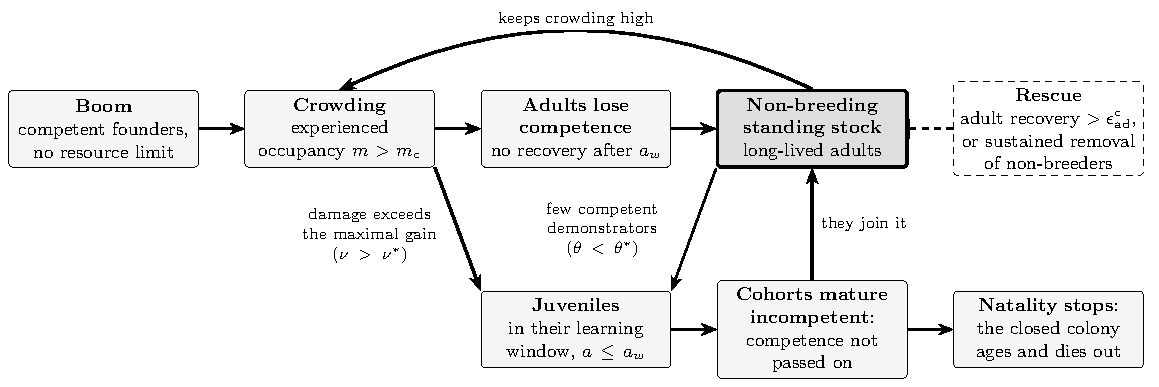
\includegraphics[width=\textwidth]{fig_causal.pdf}
  \caption{Causal scheme of the collapse. Thick arrows form the reinforcing loop. Crowding makes adults lose their
  reproductive competence. After the sensitive window ($a>a_w$) the loss is permanent, and the long-lived
  non-breeders (a standing stock of non-breeding adults) keep crowding high: in space during the
  aggregated growth, in the well-mixed limit by holding the density above $\nu^*$ (sufficiency conjectural;
  Section~\ref{sec:res-mechanism}). Juveniles in their window are then damaged faster than they can learn. They
  also learn from few competent demonstrators ($\theta<\theta^*$, a precursor), so they mature incompetent and join
  the standing stock, and natality stops. Whether adults recover is the condition of the mechanism (dashed): above a
  threshold $\eadult^c$ of adult recovery the colony persists (Fig.~\ref{fig:recovery}); a sustained removal of
  non-breeders also rescues it. Protecting only the juveniles, with perfect demonstrators or a crowding-free
  nursery, does not (798 of 800 colonies went extinct; SM, Section~\ref{SM-supp:recovery}). Every step acts on
  individuals.}
  \label{fig:causal}
\end{figure}
